\documentclass[]{article}
\usepackage{lmodern}
\usepackage{amssymb,amsmath}
\usepackage{ifxetex,ifluatex}
\usepackage{fixltx2e} % provides \textsubscript
\ifnum 0\ifxetex 1\fi\ifluatex 1\fi=0 % if pdftex
  \usepackage[T1]{fontenc}
  \usepackage[utf8]{inputenc}
\else % if luatex or xelatex
  \ifxetex
    \usepackage{mathspec}
  \else
    \usepackage{fontspec}
  \fi
  \defaultfontfeatures{Ligatures=TeX,Scale=MatchLowercase}
\fi
% use upquote if available, for straight quotes in verbatim environments
\IfFileExists{upquote.sty}{\usepackage{upquote}}{}
% use microtype if available
\IfFileExists{microtype.sty}{%
\usepackage{microtype}
\UseMicrotypeSet[protrusion]{basicmath} % disable protrusion for tt fonts
}{}
\usepackage[margin=1in]{geometry}
\usepackage{hyperref}
\hypersetup{unicode=true,
            pdftitle={MoTrPAC: power calculations for mixed effects datasets with time},
            pdfauthor={David Amar},
            pdfborder={0 0 0},
            breaklinks=true}
\urlstyle{same}  % don't use monospace font for urls
\usepackage{color}
\usepackage{fancyvrb}
\newcommand{\VerbBar}{|}
\newcommand{\VERB}{\Verb[commandchars=\\\{\}]}
\DefineVerbatimEnvironment{Highlighting}{Verbatim}{commandchars=\\\{\}}
% Add ',fontsize=\small' for more characters per line
\usepackage{framed}
\definecolor{shadecolor}{RGB}{248,248,248}
\newenvironment{Shaded}{\begin{snugshade}}{\end{snugshade}}
\newcommand{\KeywordTok}[1]{\textcolor[rgb]{0.13,0.29,0.53}{\textbf{#1}}}
\newcommand{\DataTypeTok}[1]{\textcolor[rgb]{0.13,0.29,0.53}{#1}}
\newcommand{\DecValTok}[1]{\textcolor[rgb]{0.00,0.00,0.81}{#1}}
\newcommand{\BaseNTok}[1]{\textcolor[rgb]{0.00,0.00,0.81}{#1}}
\newcommand{\FloatTok}[1]{\textcolor[rgb]{0.00,0.00,0.81}{#1}}
\newcommand{\ConstantTok}[1]{\textcolor[rgb]{0.00,0.00,0.00}{#1}}
\newcommand{\CharTok}[1]{\textcolor[rgb]{0.31,0.60,0.02}{#1}}
\newcommand{\SpecialCharTok}[1]{\textcolor[rgb]{0.00,0.00,0.00}{#1}}
\newcommand{\StringTok}[1]{\textcolor[rgb]{0.31,0.60,0.02}{#1}}
\newcommand{\VerbatimStringTok}[1]{\textcolor[rgb]{0.31,0.60,0.02}{#1}}
\newcommand{\SpecialStringTok}[1]{\textcolor[rgb]{0.31,0.60,0.02}{#1}}
\newcommand{\ImportTok}[1]{#1}
\newcommand{\CommentTok}[1]{\textcolor[rgb]{0.56,0.35,0.01}{\textit{#1}}}
\newcommand{\DocumentationTok}[1]{\textcolor[rgb]{0.56,0.35,0.01}{\textbf{\textit{#1}}}}
\newcommand{\AnnotationTok}[1]{\textcolor[rgb]{0.56,0.35,0.01}{\textbf{\textit{#1}}}}
\newcommand{\CommentVarTok}[1]{\textcolor[rgb]{0.56,0.35,0.01}{\textbf{\textit{#1}}}}
\newcommand{\OtherTok}[1]{\textcolor[rgb]{0.56,0.35,0.01}{#1}}
\newcommand{\FunctionTok}[1]{\textcolor[rgb]{0.00,0.00,0.00}{#1}}
\newcommand{\VariableTok}[1]{\textcolor[rgb]{0.00,0.00,0.00}{#1}}
\newcommand{\ControlFlowTok}[1]{\textcolor[rgb]{0.13,0.29,0.53}{\textbf{#1}}}
\newcommand{\OperatorTok}[1]{\textcolor[rgb]{0.81,0.36,0.00}{\textbf{#1}}}
\newcommand{\BuiltInTok}[1]{#1}
\newcommand{\ExtensionTok}[1]{#1}
\newcommand{\PreprocessorTok}[1]{\textcolor[rgb]{0.56,0.35,0.01}{\textit{#1}}}
\newcommand{\AttributeTok}[1]{\textcolor[rgb]{0.77,0.63,0.00}{#1}}
\newcommand{\RegionMarkerTok}[1]{#1}
\newcommand{\InformationTok}[1]{\textcolor[rgb]{0.56,0.35,0.01}{\textbf{\textit{#1}}}}
\newcommand{\WarningTok}[1]{\textcolor[rgb]{0.56,0.35,0.01}{\textbf{\textit{#1}}}}
\newcommand{\AlertTok}[1]{\textcolor[rgb]{0.94,0.16,0.16}{#1}}
\newcommand{\ErrorTok}[1]{\textcolor[rgb]{0.64,0.00,0.00}{\textbf{#1}}}
\newcommand{\NormalTok}[1]{#1}
\usepackage{graphicx,grffile}
\makeatletter
\def\maxwidth{\ifdim\Gin@nat@width>\linewidth\linewidth\else\Gin@nat@width\fi}
\def\maxheight{\ifdim\Gin@nat@height>\textheight\textheight\else\Gin@nat@height\fi}
\makeatother
% Scale images if necessary, so that they will not overflow the page
% margins by default, and it is still possible to overwrite the defaults
% using explicit options in \includegraphics[width, height, ...]{}
\setkeys{Gin}{width=\maxwidth,height=\maxheight,keepaspectratio}
\IfFileExists{parskip.sty}{%
\usepackage{parskip}
}{% else
\setlength{\parindent}{0pt}
\setlength{\parskip}{6pt plus 2pt minus 1pt}
}
\setlength{\emergencystretch}{3em}  % prevent overfull lines
\providecommand{\tightlist}{%
  \setlength{\itemsep}{0pt}\setlength{\parskip}{0pt}}
\setcounter{secnumdepth}{0}
% Redefines (sub)paragraphs to behave more like sections
\ifx\paragraph\undefined\else
\let\oldparagraph\paragraph
\renewcommand{\paragraph}[1]{\oldparagraph{#1}\mbox{}}
\fi
\ifx\subparagraph\undefined\else
\let\oldsubparagraph\subparagraph
\renewcommand{\subparagraph}[1]{\oldsubparagraph{#1}\mbox{}}
\fi

%%% Use protect on footnotes to avoid problems with footnotes in titles
\let\rmarkdownfootnote\footnote%
\def\footnote{\protect\rmarkdownfootnote}

%%% Change title format to be more compact
\usepackage{titling}

% Create subtitle command for use in maketitle
\newcommand{\subtitle}[1]{
  \posttitle{
    \begin{center}\large#1\end{center}
    }
}

\setlength{\droptitle}{-2em}
  \title{MoTrPAC: power calculations for mixed effects datasets with time}
  \pretitle{\vspace{\droptitle}\centering\huge}
  \posttitle{\par}
  \author{David Amar}
  \preauthor{\centering\large\emph}
  \postauthor{\par}
  \predate{\centering\large\emph}
  \postdate{\par}
  \date{9/15/2018}

\usepackage{booktabs} \usepackage{longtable} \usepackage{array}
\usepackage{multirow} \usepackage[table]{xcolor} \usepackage{wrapfig}
\usepackage{float} \floatplacement{figure}{H}

\begin{document}
\maketitle

\section{The underlying model}\label{the-underlying-model}

We simulate linear mixed effects models with a random intercept model.
Each subject (g) has its own intercept but the subjects share a common
transient trend. There are five time points per subject: one pre- (time
point zero) and four post-exercise (time points 1-4). The transient
response peaks at the second post-exercise time point, whereas time
points 1 and 3 have 25/\% of the peak effect. The last time point has no
effect. We use the lme4 and simr R packages to calculate the detection
power for different cases. We first show example data sets with
different within vs.~between subject variability ratios. We fix the
between variance to 1 and change the within variance.

\begin{Shaded}
\begin{Highlighting}[]
\CommentTok{# Helper functions}
\CommentTok{# Simulate a linear mixed effects dataset}
\NormalTok{simulate_data<-}\ControlFlowTok{function}\NormalTok{(n_t,sigma_between,sigma_within,effects_vec,}
\NormalTok{                        n_subjects,effect_size,}\DataTypeTok{use_arima=}\NormalTok{F,}\DataTypeTok{arima_rho=}\FloatTok{0.5}\NormalTok{)\{}
\NormalTok{  intecepts =}\StringTok{ }\KeywordTok{rnorm}\NormalTok{(n_subjects,}\DataTypeTok{sd =}\NormalTok{ sigma_between)}
\NormalTok{  y =}\StringTok{ }\KeywordTok{c}\NormalTok{()}
\NormalTok{  g =}\StringTok{ }\KeywordTok{c}\NormalTok{()}
\NormalTok{  tp =}\StringTok{ }\KeywordTok{c}\NormalTok{()}
  \ControlFlowTok{for}\NormalTok{(j }\ControlFlowTok{in} \DecValTok{1}\OperatorTok{:}\NormalTok{n_subjects)\{}
\NormalTok{    errs =}\StringTok{ }\KeywordTok{rnorm}\NormalTok{(n_t,}\DataTypeTok{sd=}\NormalTok{sigma_within)}
    \ControlFlowTok{if}\NormalTok{(use_arima)\{}
\NormalTok{      errs =}\StringTok{ }\KeywordTok{arima.sim}\NormalTok{(}\KeywordTok{list}\NormalTok{(}\DataTypeTok{order =} \KeywordTok{c}\NormalTok{(}\DecValTok{1}\NormalTok{,}\DecValTok{0}\NormalTok{,}\DecValTok{0}\NormalTok{), }\DataTypeTok{ar =}\NormalTok{ arima_rho),}
                       \DataTypeTok{n =}\NormalTok{ n_t,}\DataTypeTok{sd =}\NormalTok{ sigma_within) }
\NormalTok{    \}}
\NormalTok{    effs =}\StringTok{ }\NormalTok{effect_size }\OperatorTok{*}\StringTok{ }\NormalTok{effects_vec}
\NormalTok{    y =}\StringTok{ }\KeywordTok{c}\NormalTok{(y,intecepts[j]}\OperatorTok{+}\NormalTok{errs}\OperatorTok{+}\NormalTok{effs)}
\NormalTok{    g =}\StringTok{ }\KeywordTok{c}\NormalTok{(g,}\KeywordTok{rep}\NormalTok{(j,n_t))}
\NormalTok{    tp =}\StringTok{ }\KeywordTok{c}\NormalTok{(tp,}\DecValTok{0}\OperatorTok{:}\NormalTok{(n_t}\OperatorTok{-}\DecValTok{1}\NormalTok{))}
\NormalTok{  \}}
\NormalTok{  d =}\StringTok{ }\KeywordTok{data.frame}\NormalTok{(y,g,}\DataTypeTok{t=}\NormalTok{tp)}
  \KeywordTok{return}\NormalTok{(d)}
\NormalTok{\}}
\CommentTok{# Plot the trajectories of the subjects}
\NormalTok{plot_longi<-}\ControlFlowTok{function}\NormalTok{(d,...)\{}
  \KeywordTok{plot}\NormalTok{(}\DataTypeTok{y=}\NormalTok{d}\OperatorTok{$}\NormalTok{y,d}\OperatorTok{$}\NormalTok{t,}\DataTypeTok{type=}\StringTok{"n"}\NormalTok{,}\DataTypeTok{ylab=}\StringTok{"abundance"}\NormalTok{,...)}
  \KeywordTok{points}\NormalTok{(}\DataTypeTok{y=}\NormalTok{d}\OperatorTok{$}\NormalTok{y,d}\OperatorTok{$}\NormalTok{t,}\DataTypeTok{type=}\StringTok{"p"}\NormalTok{,}\DataTypeTok{pch=}\DecValTok{3}\NormalTok{)}
  \ControlFlowTok{for}\NormalTok{(i }\ControlFlowTok{in} \KeywordTok{unique}\NormalTok{(d}\OperatorTok{$}\NormalTok{g))\{}\KeywordTok{lines}\NormalTok{(}\DataTypeTok{y=}\NormalTok{d}\OperatorTok{$}\NormalTok{y[d}\OperatorTok{$}\NormalTok{g}\OperatorTok{==}\NormalTok{i],d}\OperatorTok{$}\NormalTok{t[d}\OperatorTok{$}\NormalTok{g}\OperatorTok{==}\NormalTok{i],}\DataTypeTok{type=}\StringTok{"l"}\NormalTok{,}\DataTypeTok{lty=}\DecValTok{2}\NormalTok{)\} }
  \KeywordTok{lines}\NormalTok{(}\KeywordTok{lowess}\NormalTok{(}\DataTypeTok{y=}\NormalTok{d}\OperatorTok{$}\NormalTok{y,d}\OperatorTok{$}\NormalTok{t,}\DataTypeTok{f=}\FloatTok{0.1}\NormalTok{),}\DataTypeTok{lwd=}\DecValTok{3}\NormalTok{,}\DataTypeTok{col=}\StringTok{"yellow"}\NormalTok{) }
\NormalTok{\}}

\CommentTok{# Example dataset:}
\NormalTok{n_t =}\StringTok{ }\DecValTok{5} \CommentTok{# one for pre and then four time points}
\NormalTok{sigma_between =}\StringTok{ }\DecValTok{2} \CommentTok{# random effect standard deviation}
\NormalTok{n_subjects =}\StringTok{ }\DecValTok{50}
\NormalTok{effects_vec =}\StringTok{ }\KeywordTok{c}\NormalTok{(}\DecValTok{0}\NormalTok{,}\FloatTok{0.25}\NormalTok{,}\DecValTok{1}\NormalTok{,}\FloatTok{0.25}\NormalTok{,}\DecValTok{0}\NormalTok{)}
\NormalTok{effect_size =}\StringTok{ }\DecValTok{1}
\KeywordTok{par}\NormalTok{(}\DataTypeTok{mfrow=}\KeywordTok{c}\NormalTok{(}\DecValTok{1}\NormalTok{,}\DecValTok{3}\NormalTok{))}
\NormalTok{sigma_within =}\StringTok{ }\DecValTok{1}
\NormalTok{d =}\StringTok{ }\KeywordTok{simulate_data}\NormalTok{(n_t,sigma_between,sigma_within ,effects_vec,n_subjects,effect_size)}
\KeywordTok{plot_longi}\NormalTok{(d,}\DataTypeTok{xlab=}\StringTok{"time points"}\NormalTok{,}\DataTypeTok{main=}\StringTok{"(High) Sigma within: 1"}\NormalTok{)}
\NormalTok{sigma_within =}\StringTok{ }\FloatTok{0.5}
\NormalTok{d =}\StringTok{ }\KeywordTok{simulate_data}\NormalTok{(n_t,sigma_between,sigma_within ,effects_vec,n_subjects,effect_size)}
\KeywordTok{plot_longi}\NormalTok{(d,}\DataTypeTok{xlab=}\StringTok{"time points"}\NormalTok{,}\DataTypeTok{main=}\StringTok{"(Medium) Sigma within: 0.5"}\NormalTok{)}
\NormalTok{sigma_within =}\StringTok{ }\FloatTok{0.1}
\NormalTok{d =}\StringTok{ }\KeywordTok{simulate_data}\NormalTok{(n_t,sigma_between,sigma_within ,effects_vec,n_subjects,effect_size)}
\KeywordTok{plot_longi}\NormalTok{(d,}\DataTypeTok{xlab=}\StringTok{"time points"}\NormalTok{,}\DataTypeTok{main=}\StringTok{"(Low) Sigma within: 0.1"}\NormalTok{)}
\end{Highlighting}
\end{Shaded}

\begin{figure}
\centering
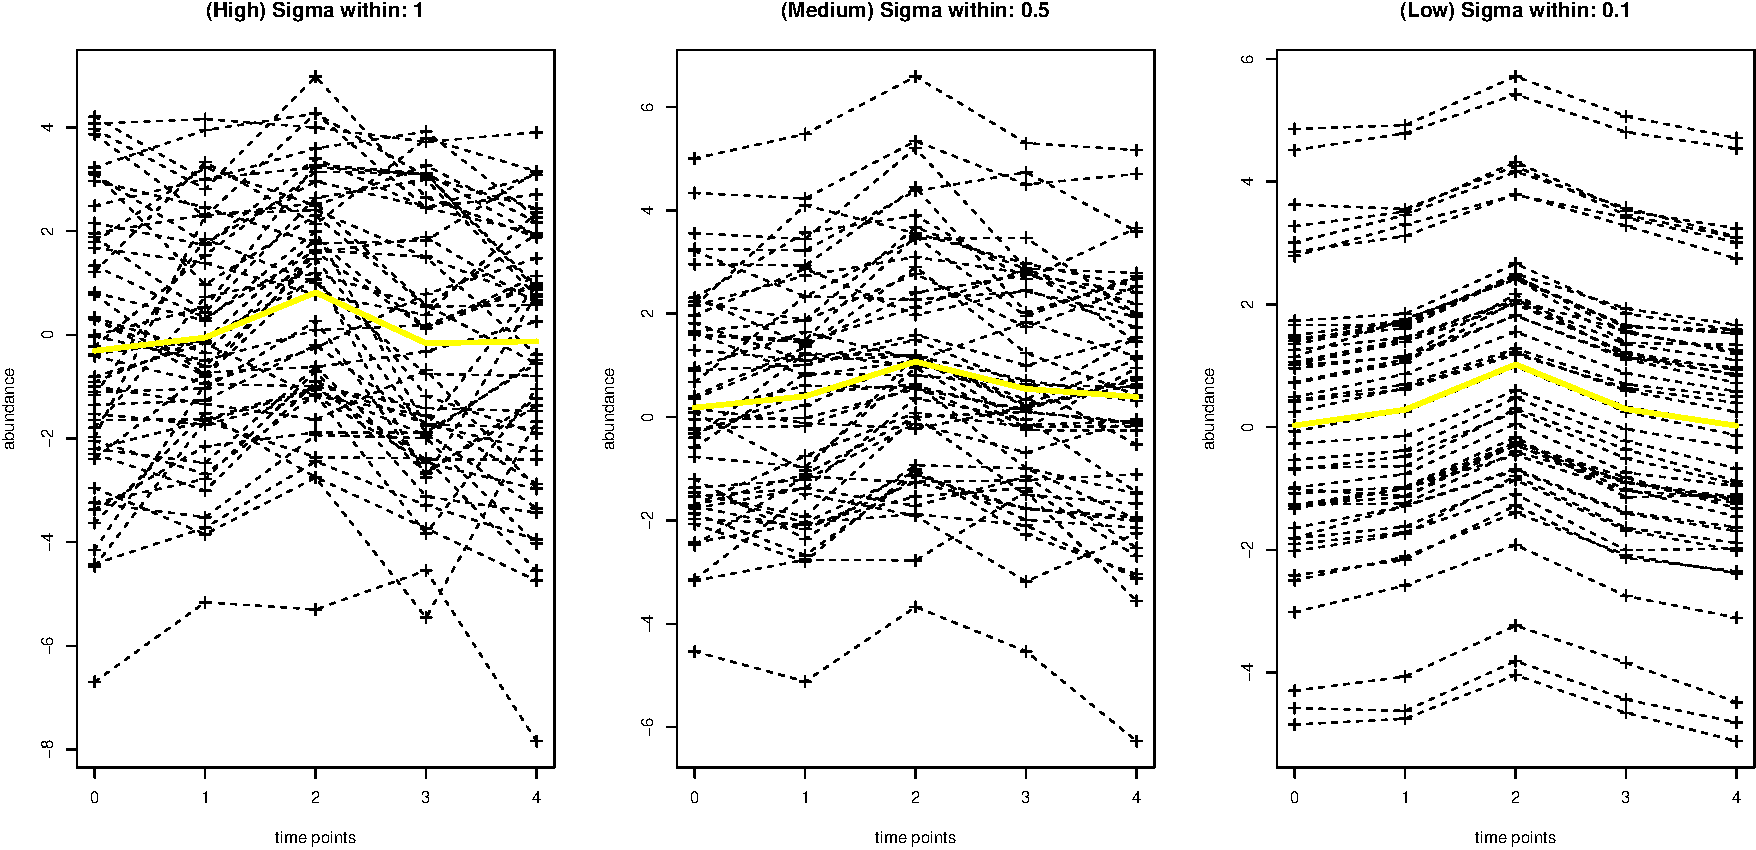
\includegraphics{power_calculations_files/figure-latex/funcs-1.pdf}
\caption{Simulated data examples with different within variance
parameters. Greate values lead to a `noisy' plot. Yellow lines represent
the average time reponse.}
\end{figure}

\section{Power calculation
considerations}\label{power-calculation-considerations}

Obviously, if the time response of an anlyte is transient and involves
time points that are not covered in the study then the detection power
is zero. Here, we consider power calculations for the data sets as in
Figure 1 with different within variance and effect size parameters. We
also consider two different methods for analyte discovery: (1) a naive
LMM that treats time as factors, and (2) fitting linear and cubic
orthogonal polynomials. Given our transient response, we expect that the
2-degree polynomial will detect the differential abundance pattern.
Greater degrees can be considered but were ignored because of the low
number of time points per subject. All power calculations below are for
a significance level of 0.001 (which should be close to an FDR of 0.05).

\begin{Shaded}
\begin{Highlighting}[]
\KeywordTok{library}\NormalTok{(lme4);}\KeywordTok{library}\NormalTok{(simr);}\KeywordTok{library}\NormalTok{(gplots)}
\CommentTok{#' Power analysis that treats time as simple factors}
\CommentTok{#' }
\CommentTok{#'  @param d A data frame of simulated data. For example, output of simulate_data}
\CommentTok{#'  @param effects_var A numeric vector specifying relative weights for a trajectory}
\CommentTok{#'  @param effect_size A number. the effect size to multiply effects_var by}
\CommentTok{#'  @param max_m A number.  The maximal numer of subjects to consider in calculations}
\CommentTok{#'  @param nsim A number. Number of simulations for simr}
\CommentTok{#'  @param alpha A number. The significance level for the power calculations}
\CommentTok{#'  @param tp A number. The time point of interest. The power calculation focuses on }
\CommentTok{#'  the ability to detect the effect in this time point}
\CommentTok{#'  @param ... additional parameters to powerCurve (simr)}
\CommentTok{#'  }
\CommentTok{#'  @return A power curve}
\NormalTok{get_simple_power_plot<-}\ControlFlowTok{function}\NormalTok{(d,effects_vec,effect_size,}
                                \DataTypeTok{max_n=}\DecValTok{700}\NormalTok{,}\DataTypeTok{nsim=}\DecValTok{10}\NormalTok{,}\DataTypeTok{alpha=}\FloatTok{0.001}\NormalTok{,}\DataTypeTok{tp=}\DecValTok{1}\NormalTok{,...)\{}
\NormalTok{  simr_model =}\StringTok{ }\KeywordTok{lmer}\NormalTok{(y}\OperatorTok{~}\KeywordTok{factor}\NormalTok{(t)}\OperatorTok{+}\NormalTok{(}\DecValTok{1}\OperatorTok{|}\NormalTok{g),}\DataTypeTok{data=}\NormalTok{d)}
  \CommentTok{# specify desired effect sizes}
  \ControlFlowTok{for}\NormalTok{(j }\ControlFlowTok{in} \DecValTok{2}\OperatorTok{:}\NormalTok{n_t)\{}
    \KeywordTok{fixef}\NormalTok{(simr_model)[}\KeywordTok{paste}\NormalTok{(}\StringTok{"factor(t)"}\NormalTok{,j}\OperatorTok{-}\DecValTok{1}\NormalTok{,}\DataTypeTok{sep=}\StringTok{""}\NormalTok{)] =}\StringTok{ }\NormalTok{effects_vec[j]}\OperatorTok{*}\NormalTok{effect_size}
\NormalTok{  \}}
  \CommentTok{# Analysis at a range of sample sizes}
\NormalTok{  model3 <-}\StringTok{ }\KeywordTok{extend}\NormalTok{(simr_model, }\DataTypeTok{along=}\StringTok{"g"}\NormalTok{, }\DataTypeTok{n=}\NormalTok{max_n)}
\NormalTok{  pc3 <-}\StringTok{ }\KeywordTok{powerCurve}\NormalTok{(model3, }\DataTypeTok{along=}\StringTok{"g"}\NormalTok{,}
                    \DataTypeTok{test=}\KeywordTok{fixed}\NormalTok{(}\KeywordTok{paste}\NormalTok{(}\StringTok{"factor(t)"}\NormalTok{,tp,}\DataTypeTok{sep=}\StringTok{""}\NormalTok{),}\StringTok{"z"}\NormalTok{),}
                    \DataTypeTok{alpha=}\NormalTok{alpha,}\DataTypeTok{nsim=}\NormalTok{nsim,...)}
  \KeywordTok{return}\NormalTok{(pc3)}
\NormalTok{\}}

\CommentTok{#' Power analysis that uses polynomials to model time trajectories.}
\CommentTok{#' }
\CommentTok{#'  @param d A data frame of simulated data. For example, output of simulate_data}
\CommentTok{#'  @param effects_var A numeric vector specifying relative weights for a trajectory}
\CommentTok{#'  @param effect_size A number. the effect size to multiply effects_var by}
\CommentTok{#'  @param max_m A number.  The maximal numer of subjects to consider in calculations}
\CommentTok{#'  @param nsim A number. Number of simulations for simr}
\CommentTok{#'  @param alpha A number. The significance level for the power calculations}
\CommentTok{#'  @param poly_deg A number. The polynomial degree. The power calculation focuses on }
\CommentTok{#'  the ability to detect the effect in this trajectory type}
\CommentTok{#'  @param ... additional parameters to powerCurve (simr)}
\CommentTok{#'  }
\CommentTok{#'  @return A power curve}
\NormalTok{get_poly_power_plot<-}\ControlFlowTok{function}\NormalTok{(d,effects_vec,effect_size,}
                              \DataTypeTok{max_n=}\DecValTok{700}\NormalTok{,}\DataTypeTok{nsim=}\DecValTok{10}\NormalTok{,}\DataTypeTok{alpha=}\FloatTok{0.001}\NormalTok{,}\DataTypeTok{poly_deg=}\DecValTok{2}\NormalTok{,...)\{}
\NormalTok{ n_t =}\StringTok{ }\KeywordTok{length}\NormalTok{(}\KeywordTok{unique}\NormalTok{(d}\OperatorTok{$}\NormalTok{t)) }
\NormalTok{ pp =}\StringTok{ }\KeywordTok{poly}\NormalTok{(}\DecValTok{0}\OperatorTok{:}\NormalTok{(n_t}\OperatorTok{-}\DecValTok{1}\NormalTok{),}\DecValTok{2}\NormalTok{)}
\NormalTok{ yy =}\StringTok{ }\NormalTok{effects_vec}\OperatorTok{*}\NormalTok{effect_size}
\NormalTok{ new_effects_vec =}\StringTok{ }\KeywordTok{lm}\NormalTok{(yy}\OperatorTok{~}\NormalTok{pp)}\OperatorTok{$}\NormalTok{coefficients[}\OperatorTok{-}\DecValTok{1}\NormalTok{]}
 \KeywordTok{rownames}\NormalTok{(pp) =}\StringTok{ }\KeywordTok{as.character}\NormalTok{(}\DecValTok{0}\OperatorTok{:}\NormalTok{(n_t}\OperatorTok{-}\DecValTok{1}\NormalTok{))}
\NormalTok{ d_pp =}\StringTok{ }\NormalTok{pp[}\KeywordTok{as.character}\NormalTok{(d}\OperatorTok{$}\NormalTok{t),]}
 \KeywordTok{rownames}\NormalTok{(d_pp) =}\StringTok{ }\OtherTok{NULL}
\NormalTok{ d =}\StringTok{ }\KeywordTok{data.frame}\NormalTok{(d,d_pp)}
\NormalTok{ model =}\StringTok{ }\KeywordTok{lmer}\NormalTok{(y}\OperatorTok{~}\NormalTok{X1}\OperatorTok{+}\NormalTok{X2}\OperatorTok{+}\NormalTok{(}\DecValTok{1}\OperatorTok{|}\NormalTok{g),}\DataTypeTok{data=}\NormalTok{d)}
\NormalTok{ fnames =}\StringTok{ }\KeywordTok{summary}\NormalTok{(model)}\OperatorTok{$}\NormalTok{coefficients}
\NormalTok{ fnames =}\StringTok{ }\KeywordTok{rownames}\NormalTok{(fnames)[}\OperatorTok{-}\DecValTok{1}\NormalTok{]}
\NormalTok{ simr_model =}\StringTok{ }\NormalTok{model}
 \CommentTok{# specify desired effect sizes}
 \ControlFlowTok{for}\NormalTok{(j }\ControlFlowTok{in} \DecValTok{1}\OperatorTok{:}\KeywordTok{length}\NormalTok{(fnames))\{}\KeywordTok{fixef}\NormalTok{(simr_model)[fnames[j]] =}\StringTok{ }\NormalTok{new_effects_vec[j]\}}
 \CommentTok{# Analysis at a range of sample sizes}
\NormalTok{ model3 <-}\StringTok{ }\KeywordTok{extend}\NormalTok{(simr_model, }\DataTypeTok{along=}\StringTok{"g"}\NormalTok{, }\DataTypeTok{n=}\NormalTok{max_n)}
\NormalTok{ pc3 <-}\StringTok{ }\KeywordTok{powerCurve}\NormalTok{(model3, }\DataTypeTok{along=}\StringTok{"g"}\NormalTok{,}
                   \DataTypeTok{test=}\KeywordTok{fixed}\NormalTok{(fnames[poly_deg],}\StringTok{"z"}\NormalTok{),}
                   \DataTypeTok{alpha=}\NormalTok{alpha,}\DataTypeTok{nsim=}\NormalTok{nsim,...)}
 \KeywordTok{return}\NormalTok{(pc3)}
\NormalTok{\}}

\CommentTok{#' Auxiliary function for plotting power curves with errors.}
\CommentTok{#' }
\CommentTok{#'  @param l A list of powerCurve objects}
\CommentTok{#'  @param cols A vector of colors, length(cols)>=length(l)}
\CommentTok{#'  @param cols A vector of pch codes, length(pchs)>=length(l)}
\CommentTok{#'  @param ... Additional paramaters for legend}
\NormalTok{plot_ci_results<-}\ControlFlowTok{function}\NormalTok{(l,}\DataTypeTok{cols =} \KeywordTok{c}\NormalTok{(}\StringTok{"red"}\NormalTok{,}\StringTok{"green"}\NormalTok{,}\StringTok{"blue"}\NormalTok{),}\DataTypeTok{pchs=}\DecValTok{20}\OperatorTok{:}\DecValTok{24}\NormalTok{,}
                          \DataTypeTok{xlab=}\StringTok{"Number of subjects"}\NormalTok{,...)\{}
  \ControlFlowTok{if}\NormalTok{(}\KeywordTok{class}\NormalTok{(l[[}\DecValTok{1}\NormalTok{]])[}\DecValTok{1}\NormalTok{]}\OperatorTok{==}\StringTok{"powerCurve"}\NormalTok{)\{l =}\StringTok{ }\KeywordTok{lapply}\NormalTok{(l,summary)\}}
  \KeywordTok{plot}\NormalTok{(l[[}\DecValTok{1}\NormalTok{]][,}\DecValTok{1}\NormalTok{], l[[}\DecValTok{1}\NormalTok{]][,}\DecValTok{4}\NormalTok{],}\DataTypeTok{ylim=}\KeywordTok{c}\NormalTok{(}\DecValTok{0}\NormalTok{,}\FloatTok{1.2}\NormalTok{),}\DataTypeTok{type=}\StringTok{"b"}\NormalTok{,}\DataTypeTok{col=}\NormalTok{cols[}\DecValTok{1}\NormalTok{],}\DataTypeTok{pch=}\NormalTok{pchs[}\DecValTok{1}\NormalTok{],}
       \DataTypeTok{xlab=}\NormalTok{xlab,}\DataTypeTok{ylab=}\StringTok{"power"}\NormalTok{)}
  \ControlFlowTok{for}\NormalTok{(j }\ControlFlowTok{in} \DecValTok{1}\OperatorTok{:}\KeywordTok{length}\NormalTok{(l))\{}
\NormalTok{    x =}\StringTok{ }\NormalTok{l[[j]][,}\DecValTok{1}\NormalTok{]}
\NormalTok{    ui =}\StringTok{ }\KeywordTok{pmin}\NormalTok{(}\DecValTok{1}\NormalTok{,l[[j]][,}\DecValTok{6}\NormalTok{])}
\NormalTok{    li =}\StringTok{ }\KeywordTok{pmax}\NormalTok{(}\DecValTok{0}\NormalTok{,l[[j]][,}\DecValTok{5}\NormalTok{])}
    \KeywordTok{arrows}\NormalTok{(x, li, x, ui, }\DataTypeTok{length=}\FloatTok{0.05}\NormalTok{, }\DataTypeTok{angle=}\DecValTok{90}\NormalTok{, }\DataTypeTok{code=}\DecValTok{3}\NormalTok{,}\DataTypeTok{col=}\NormalTok{cols[j])  }
    \ControlFlowTok{if}\NormalTok{(j}\OperatorTok{>}\DecValTok{1}\NormalTok{)\{}
      \KeywordTok{lines}\NormalTok{(l[[j]][,}\DecValTok{1}\NormalTok{], l[[j]][,}\DecValTok{4}\NormalTok{],}\DataTypeTok{type=}\StringTok{"b"}\NormalTok{,}\DataTypeTok{col=}\NormalTok{cols[j],}\DataTypeTok{pch=}\NormalTok{pchs[j])}
\NormalTok{    \}}
\NormalTok{  \}}
  \KeywordTok{abline}\NormalTok{(}\DataTypeTok{h=}\FloatTok{0.8}\NormalTok{,}\DataTypeTok{lty=}\DecValTok{2}\NormalTok{)}
  \KeywordTok{legend}\NormalTok{(}\DataTypeTok{x=}\StringTok{"topleft"}\NormalTok{,}\DataTypeTok{legend=}\KeywordTok{names}\NormalTok{(l),}\DataTypeTok{pch=}\NormalTok{pchs,}\DataTypeTok{col=}\NormalTok{cols,}\DataTypeTok{lwd=}\DecValTok{2}\NormalTok{,}\DataTypeTok{ncol=}\DecValTok{3}\NormalTok{,...)}
\NormalTok{\}}
\end{Highlighting}
\end{Shaded}

\newpage

\section{Results}\label{results}

We plot the results below. Error bars represent variance detected during
the simulations of the simr package. To avoid unnecessary code
duplication, we show only one code example (for Figure 2).

\subsection{Power curves as a function of sample
size}\label{power-curves-as-a-function-of-sample-size}

\begin{Shaded}
\begin{Highlighting}[]
\NormalTok{sigma_between =}\StringTok{ }\DecValTok{1} \CommentTok{# random effect standard deviation}
\NormalTok{n_subjects =}\StringTok{ }\DecValTok{100}
\NormalTok{sigma_within =}\StringTok{ }\DecValTok{1}
\NormalTok{effect_size =}\StringTok{ }\FloatTok{0.5}
\NormalTok{nsim =}\StringTok{ }\DecValTok{200}
\NormalTok{d =}\StringTok{ }\KeywordTok{simulate_data}\NormalTok{(n_t,sigma_between,sigma_within ,effects_vec,n_subjects,effect_size)}
\NormalTok{ps1 =}\StringTok{ }\KeywordTok{get_simple_power_plot}\NormalTok{(d,effects_vec,effect_size,}\DataTypeTok{max_n=}\DecValTok{700}\NormalTok{,}\DataTypeTok{nsim=}\NormalTok{nsim,}\DataTypeTok{alpha=}\FloatTok{0.001}\NormalTok{,}\DataTypeTok{tp=}\DecValTok{1}\NormalTok{)}
\NormalTok{ps2 =}\StringTok{ }\KeywordTok{get_simple_power_plot}\NormalTok{(d,effects_vec,effect_size,}\DataTypeTok{max_n=}\DecValTok{700}\NormalTok{,}\DataTypeTok{nsim=}\NormalTok{nsim,}\DataTypeTok{alpha=}\FloatTok{0.001}\NormalTok{,}\DataTypeTok{tp=}\DecValTok{2}\NormalTok{)}
\NormalTok{ps3 =}\StringTok{ }\KeywordTok{get_poly_power_plot}\NormalTok{(d,effects_vec,effect_size,}\DataTypeTok{max_n=}\DecValTok{700}\NormalTok{,}\DataTypeTok{nsim=}\NormalTok{nsim,}\DataTypeTok{alpha=}\FloatTok{0.001}\NormalTok{)}
\KeywordTok{plot_ci_results}\NormalTok{(}\KeywordTok{list}\NormalTok{(}\StringTok{"S:tp=2"}\NormalTok{=ps2,}\StringTok{"S:tp=1"}\NormalTok{=ps1,}\StringTok{"P:q"}\NormalTok{=ps3),}\DataTypeTok{cex=}\FloatTok{1.3}\NormalTok{)}
\end{Highlighting}
\end{Shaded}

\begin{figure}
\centering
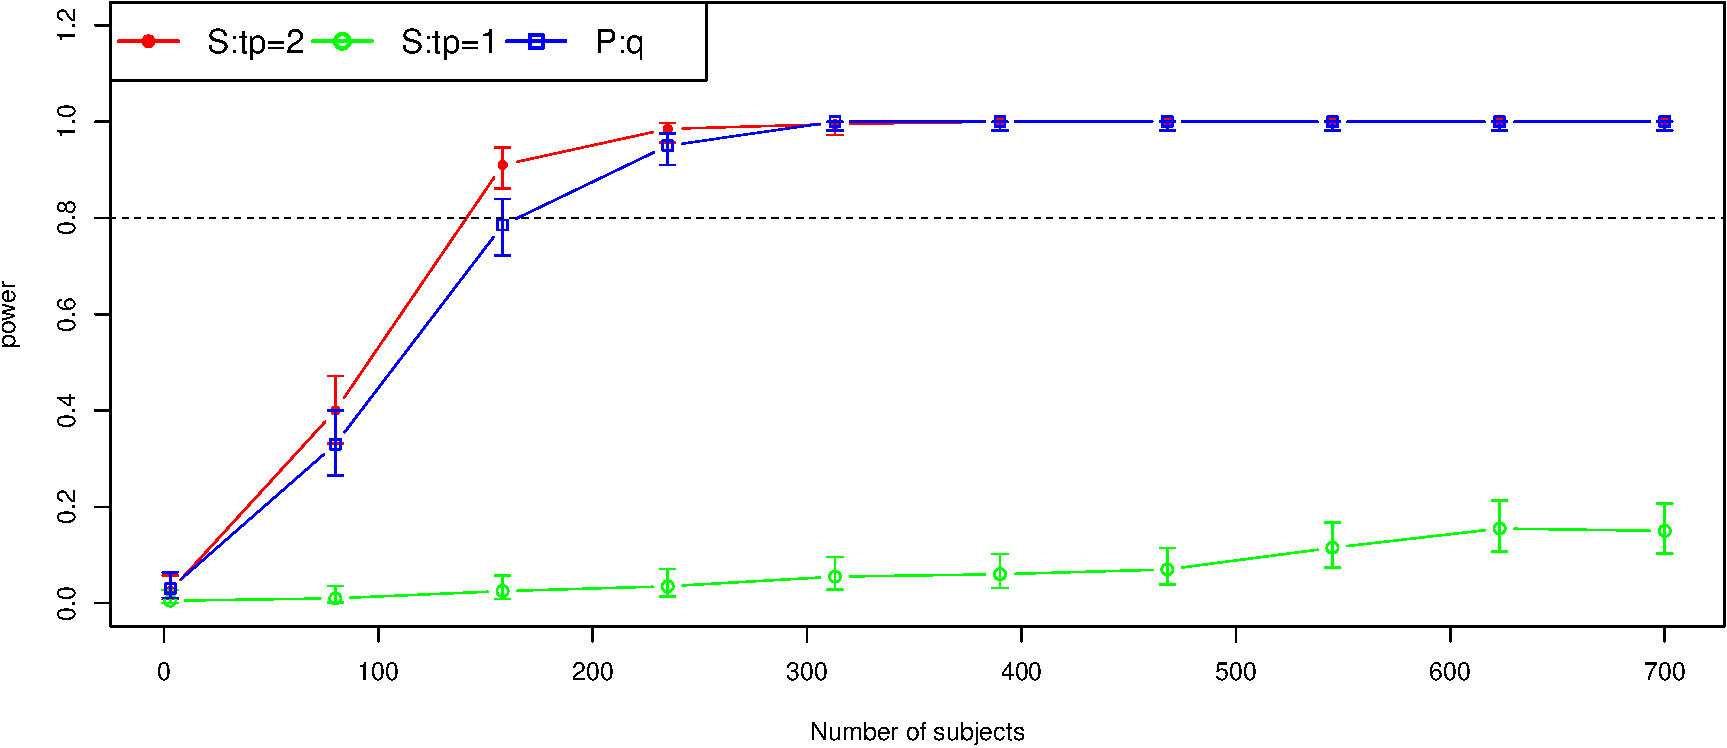
\includegraphics{power_calculations_files/figure-latex/vhigheffects1-1.pdf}
\caption{High within variance (sigma=1), peak effect size is 0.5. S
denotes the simple LMM that treats time points af factors with fixed
effects, whereas P denotes a model that fits orthogonal polynomials for
detecting the overall trend. For the simple LMM method we condifer the
power to detect either the peak effect at the second post-exercise time
point, or the previous time point with 25 percent of the peak effect.
Naturally, for this effect we get lower power.}
\end{figure}

\begin{figure}
\centering
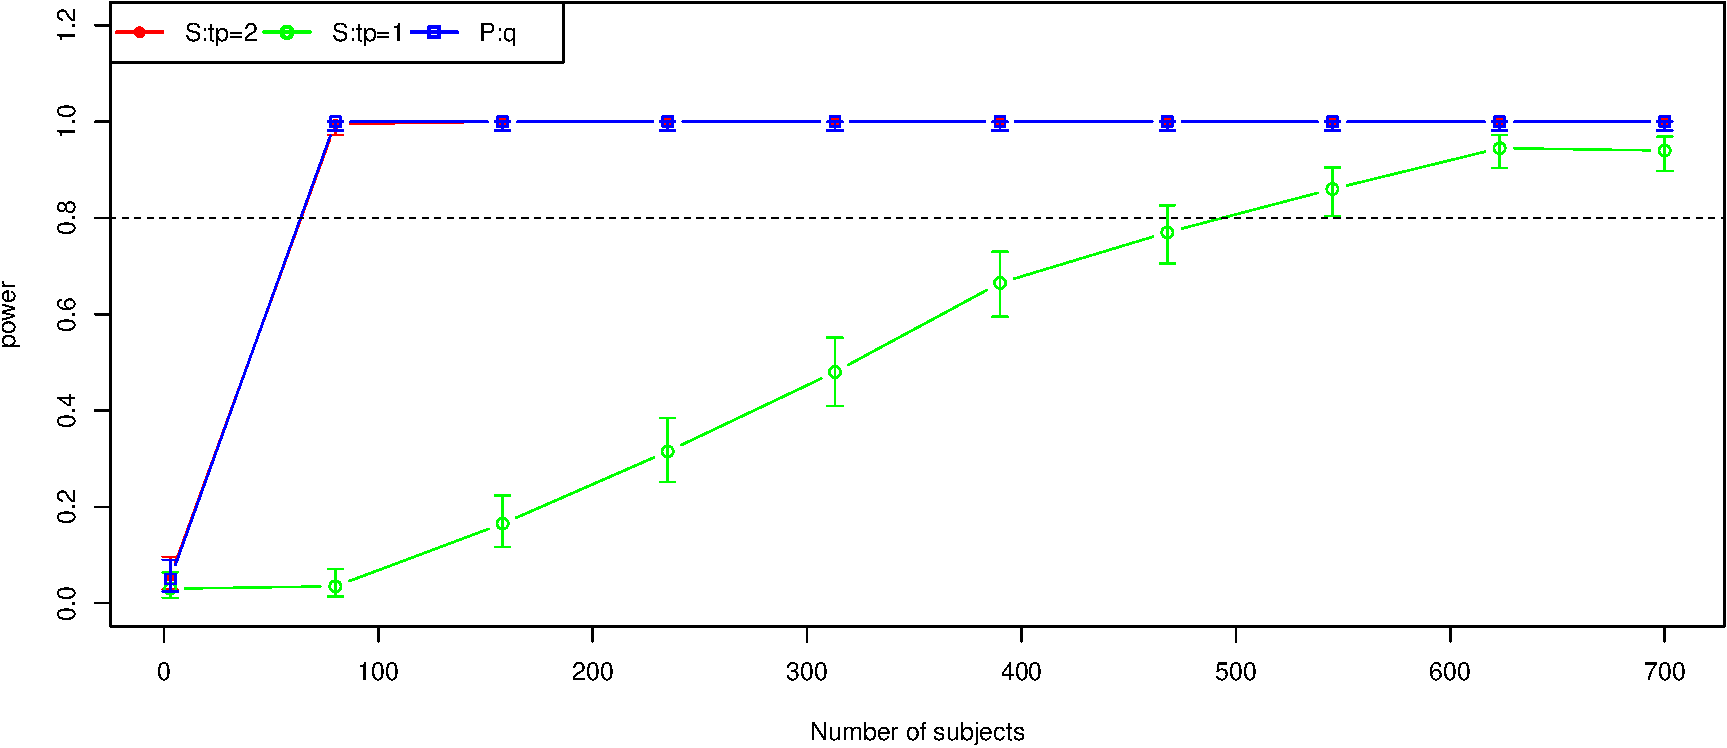
\includegraphics{power_calculations_files/figure-latex/vhigheffects2-1.pdf}
\caption{Medium within variance (sigma=0.5), peak effect size is 0.5}
\end{figure}

\begin{figure}
\centering
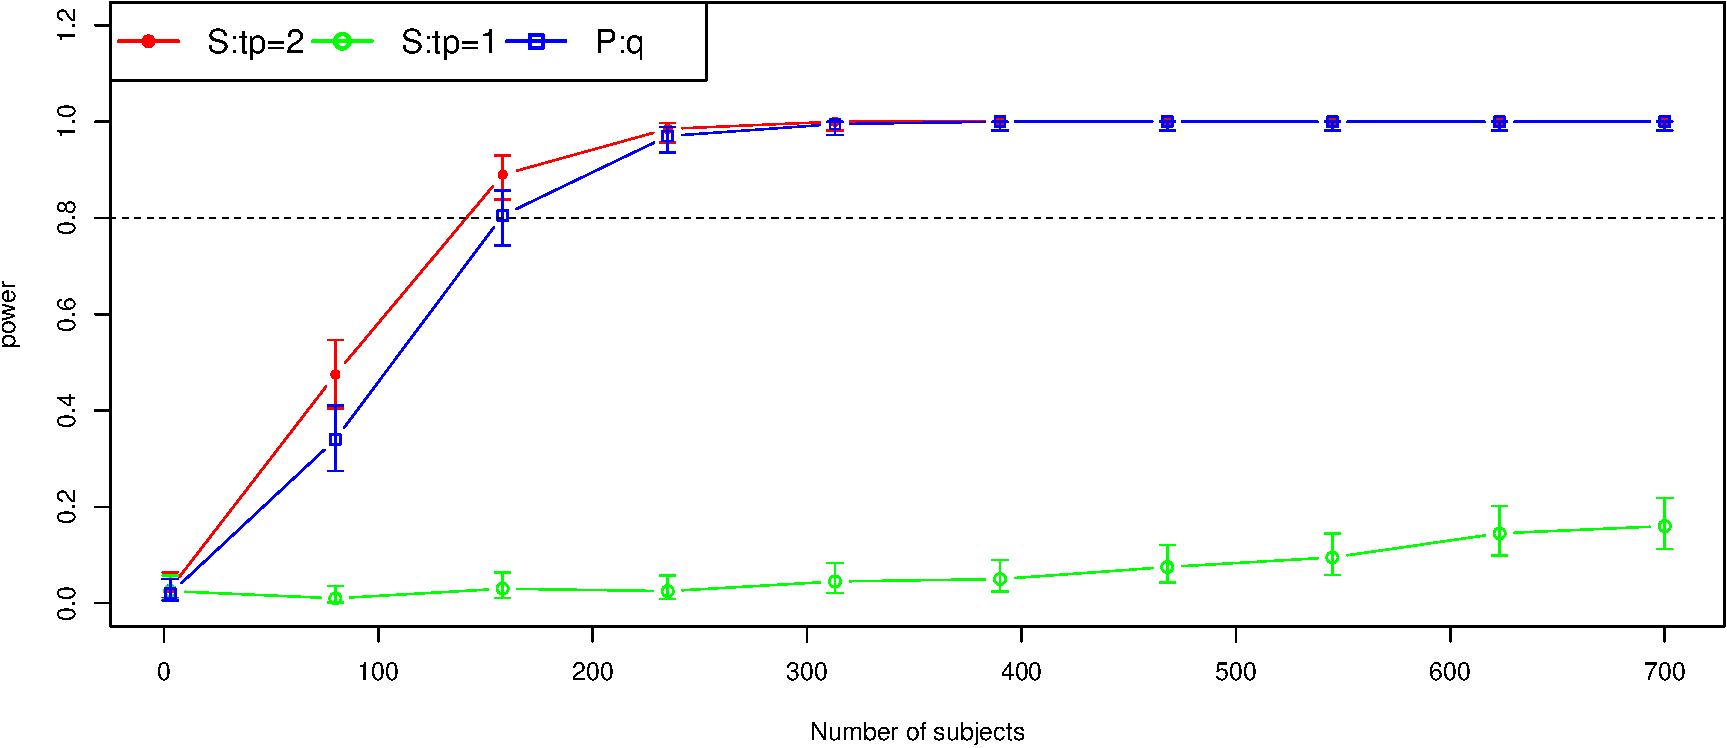
\includegraphics{power_calculations_files/figure-latex/higheffects1-1.pdf}
\caption{High within variance (sigma=1), peak effect size is 0.25.}
\end{figure}

\begin{figure}
\centering
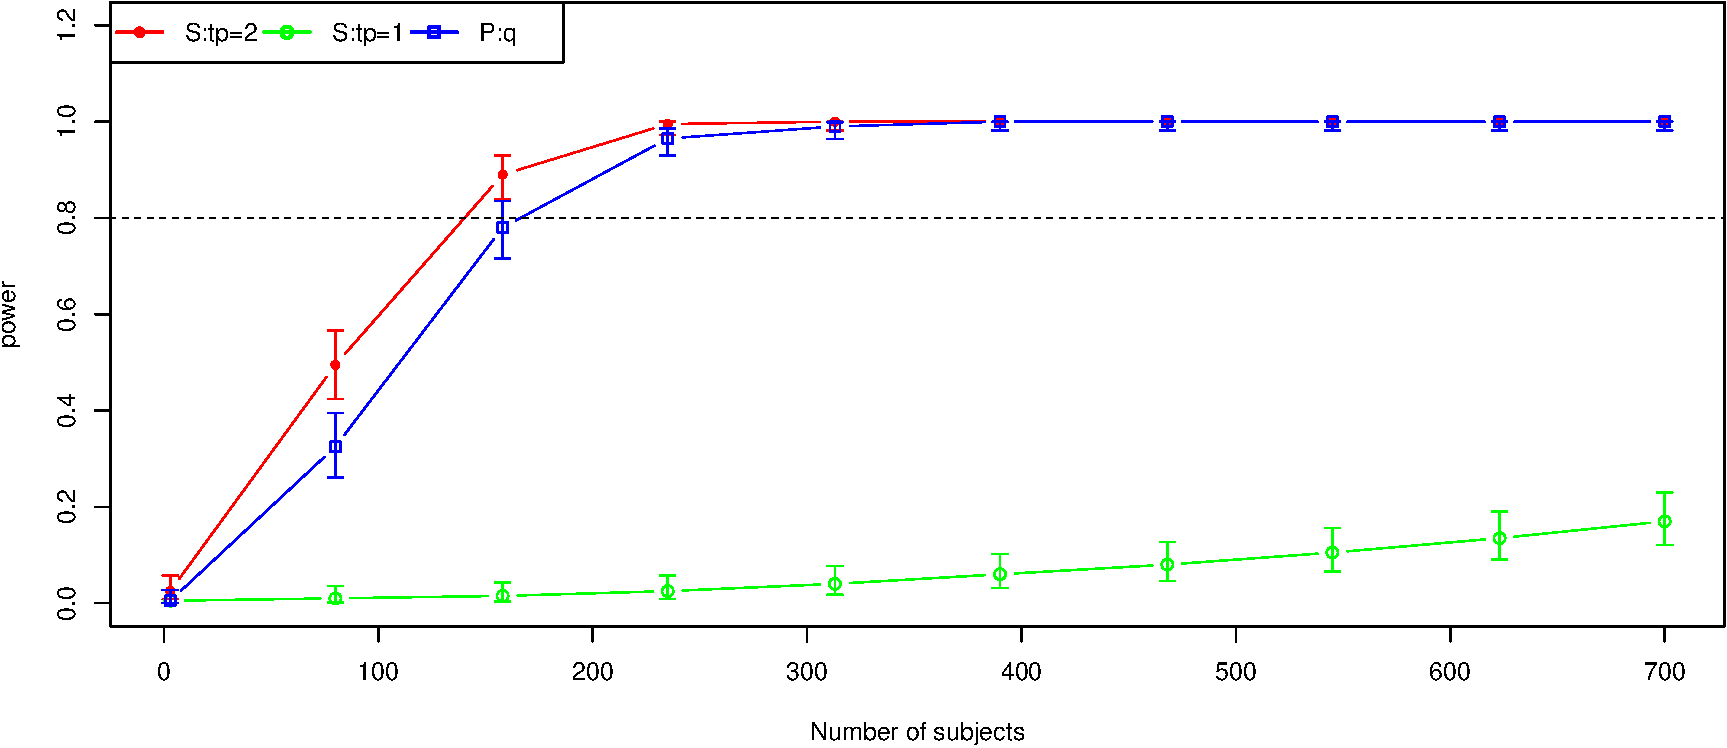
\includegraphics{power_calculations_files/figure-latex/higheffects2-1.pdf}
\caption{Medium within variance (sigma=0.5), peak effect size is 0.25}
\end{figure}

\begin{figure}
\centering
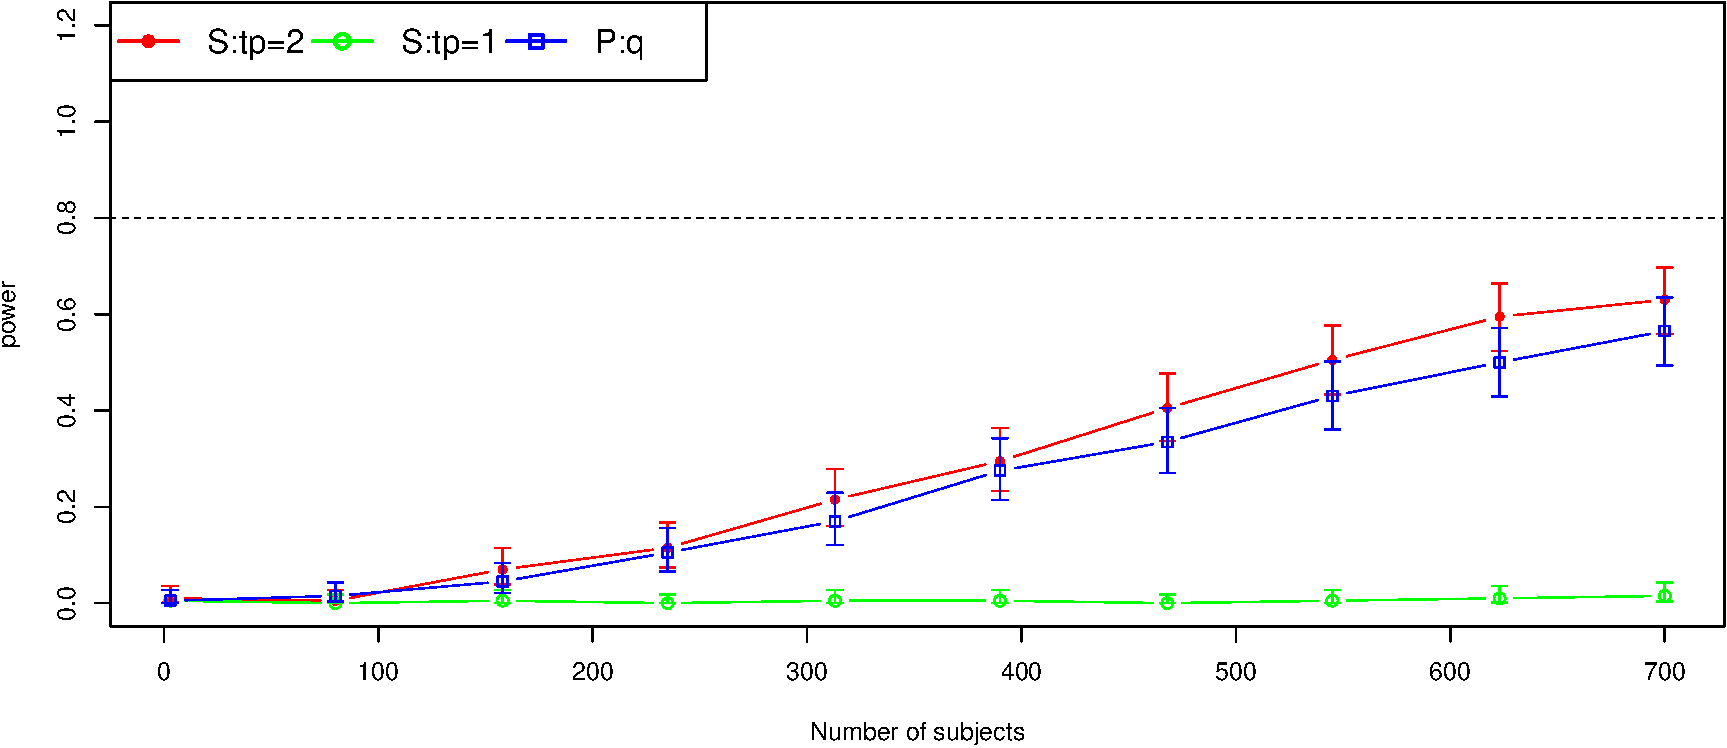
\includegraphics{power_calculations_files/figure-latex/loweffects1-1.pdf}
\caption{High within variance (sigma=1), peak effect size is 0.1}
\end{figure}

\begin{figure}
\centering
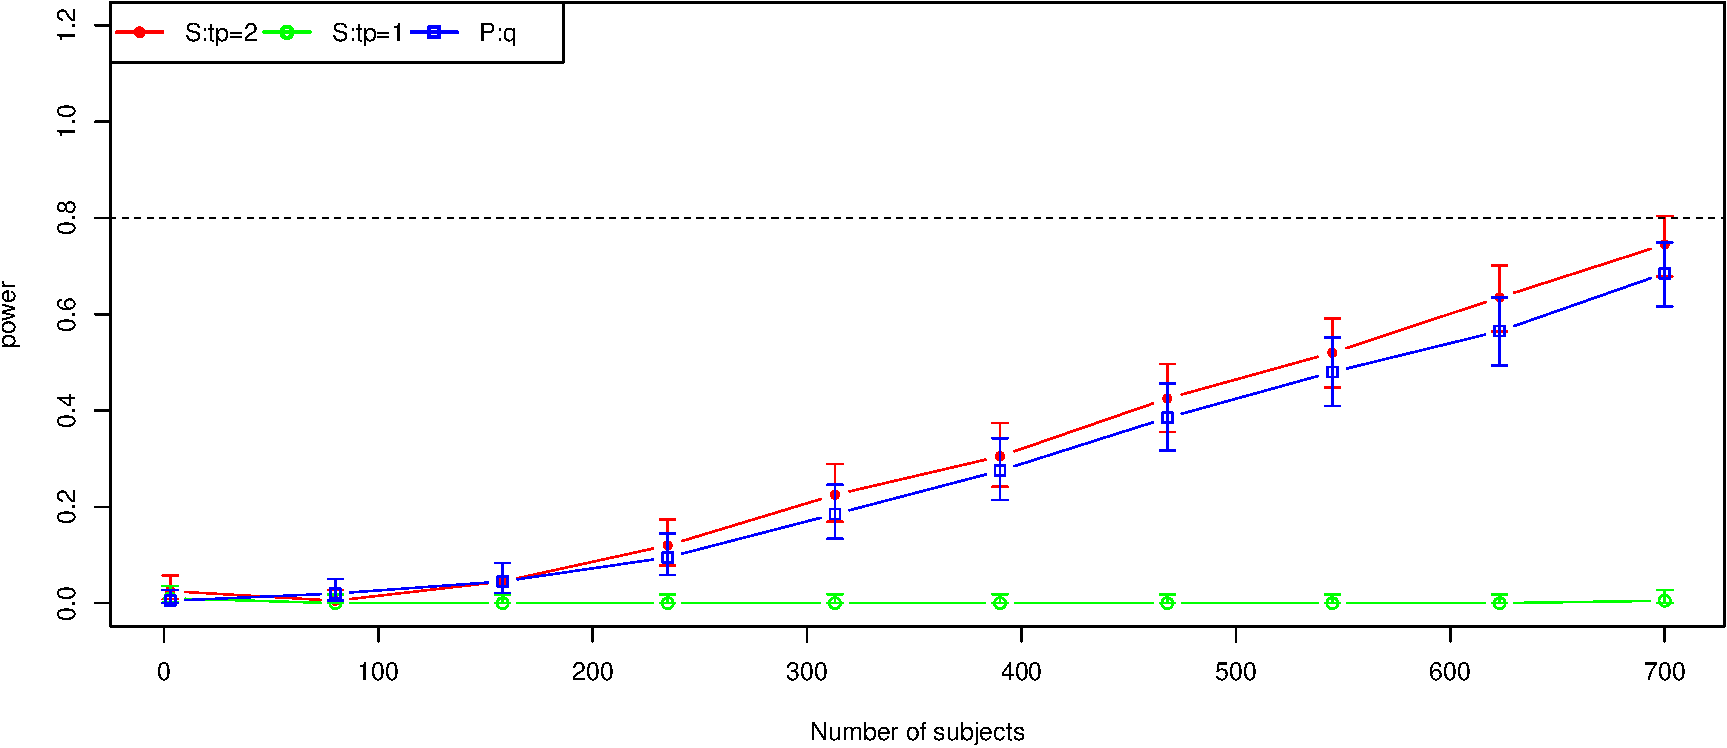
\includegraphics{power_calculations_files/figure-latex/loweffects2-1.pdf}
\caption{Medium within variance (sigma=0.5), peak effect size is 0.1}
\end{figure}

\subsection{Power curves as a function of effect
size}\label{power-curves-as-a-function-of-effect-size}

We fix the sample size to 120 and examine the power of different effect
sizes.

\begin{Shaded}
\begin{Highlighting}[]
\NormalTok{n_subjects =}\StringTok{ }\DecValTok{120}
\NormalTok{sigma_within_range =}\StringTok{ }\KeywordTok{c}\NormalTok{(}\FloatTok{0.25}\NormalTok{,}\FloatTok{0.5}\NormalTok{,}\DecValTok{1}\NormalTok{)}
\NormalTok{effect_size_range =}\StringTok{ }\KeywordTok{seq}\NormalTok{(}\FloatTok{0.1}\NormalTok{,}\DecValTok{1}\NormalTok{,}\DataTypeTok{by=}\FloatTok{0.1}\NormalTok{)}
\NormalTok{res_tp2 =}\StringTok{ }\KeywordTok{list}\NormalTok{();res_q =}\StringTok{ }\KeywordTok{list}\NormalTok{()}
\ControlFlowTok{for}\NormalTok{(sigma_within }\ControlFlowTok{in}\NormalTok{ sigma_within_range)\{}
\NormalTok{  m1 =}\StringTok{ }\KeywordTok{c}\NormalTok{();m2=}\KeywordTok{c}\NormalTok{()}
  \ControlFlowTok{for}\NormalTok{ (effect_size }\ControlFlowTok{in}\NormalTok{ effect_size_range)\{}
\NormalTok{    d =}\StringTok{ }\KeywordTok{simulate_data}\NormalTok{(n_t,sigma_between,sigma_within ,effects_vec,n_subjects,effect_size)}
\NormalTok{    ps_tp =}\StringTok{ }\KeywordTok{get_simple_power_plot}\NormalTok{(d,effects_vec,effect_size,}\DataTypeTok{max_n=}\NormalTok{n_subjects,}
                                \DataTypeTok{nsim=}\NormalTok{nsim,}\DataTypeTok{alpha=}\FloatTok{0.001}\NormalTok{,}\DataTypeTok{tp=}\DecValTok{2}\NormalTok{,}\DataTypeTok{breaks=}\NormalTok{n_subjects)}
\NormalTok{    ps_tp =}\StringTok{ }\KeywordTok{summary}\NormalTok{(ps_tp)[}\DecValTok{1}\NormalTok{,]}
\NormalTok{    ps_tp[}\DecValTok{1}\NormalTok{] =}\StringTok{ }\NormalTok{effect_size}
\NormalTok{    m1 =}\StringTok{ }\KeywordTok{rbind}\NormalTok{(m1,ps_tp)}
\NormalTok{    ps_q =}\StringTok{ }\KeywordTok{get_poly_power_plot}\NormalTok{(d,effects_vec,effect_size,}\DataTypeTok{max_n=}\NormalTok{n_subjects,}
                              \DataTypeTok{nsim=}\NormalTok{nsim,}\DataTypeTok{alpha=}\FloatTok{0.001}\NormalTok{,}\DataTypeTok{breaks=}\NormalTok{n_subjects)}
\NormalTok{    ps_q =}\StringTok{ }\KeywordTok{summary}\NormalTok{(ps_q)[}\DecValTok{1}\NormalTok{,]}
\NormalTok{    ps_q[}\DecValTok{1}\NormalTok{] =}\StringTok{ }\NormalTok{effect_size}
\NormalTok{    m2 =}\StringTok{ }\KeywordTok{rbind}\NormalTok{(m2,ps_q)}
\NormalTok{  \}}
\NormalTok{  res_tp2[[}\KeywordTok{as.character}\NormalTok{(sigma_within)]] =}\StringTok{ }\NormalTok{m1}
\NormalTok{  res_q[[}\KeywordTok{as.character}\NormalTok{(sigma_within)]] =}\StringTok{ }\NormalTok{m2}
\NormalTok{\}}
\KeywordTok{plot_ci_results}\NormalTok{(res_tp2,}\DataTypeTok{xlab=}\StringTok{"Peak effect size"}\NormalTok{)}
\end{Highlighting}
\end{Shaded}

\begin{figure}
\centering
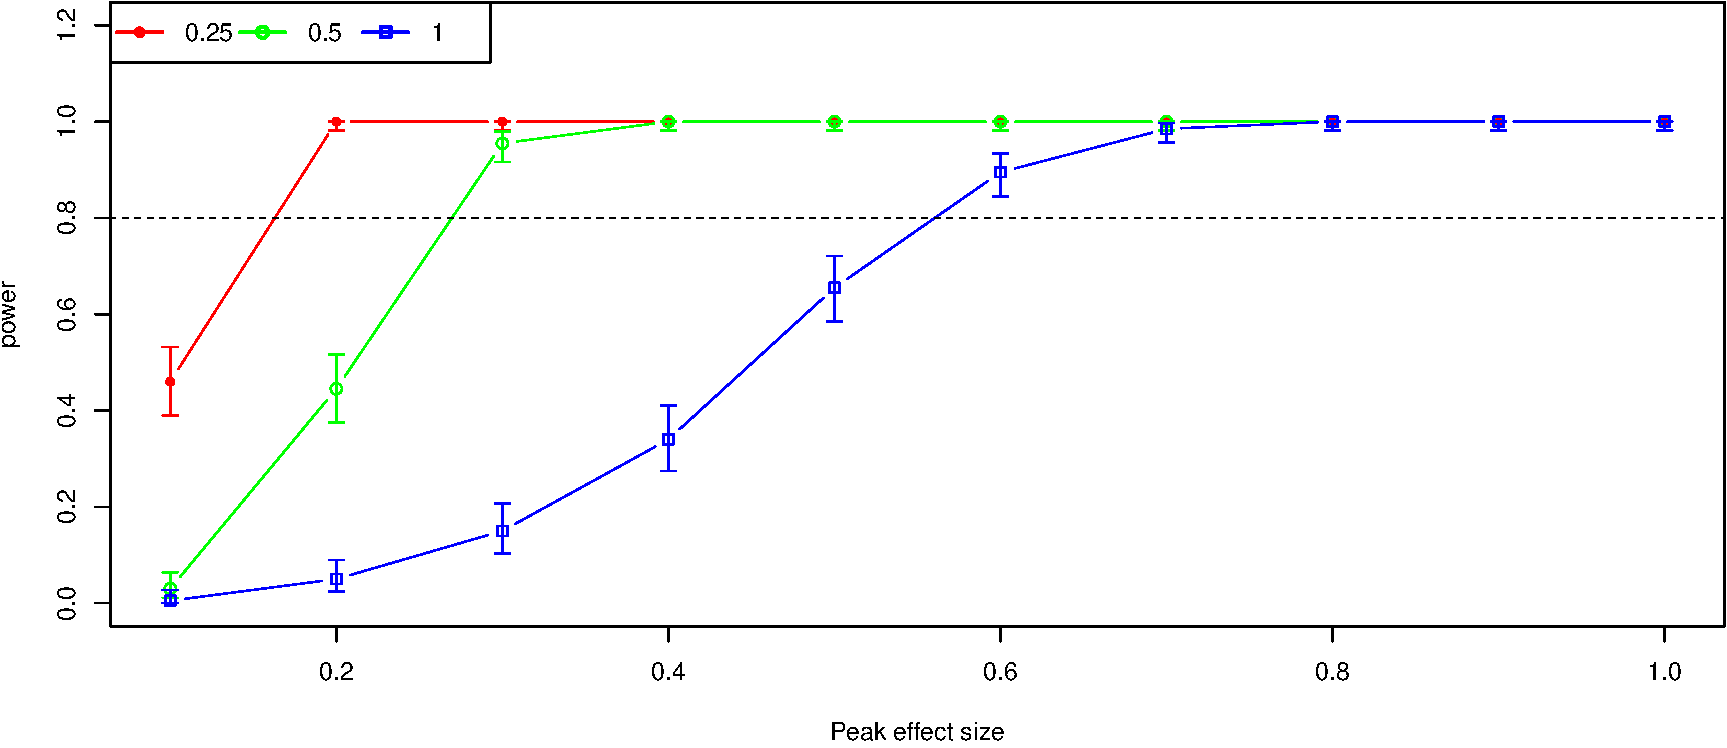
\includegraphics{power_calculations_files/figure-latex/esizes-1.pdf}
\caption{Power as a function of peak effect size when treating time as
simple factors. Number of subjects is fixed at 120. The different curves
represent different within variance.}
\end{figure}

\begin{Shaded}
\begin{Highlighting}[]
\KeywordTok{plot_ci_results}\NormalTok{(res_q,}\DataTypeTok{xlab=}\StringTok{"Peak effect size"}\NormalTok{)}
\end{Highlighting}
\end{Shaded}

\begin{figure}
\centering
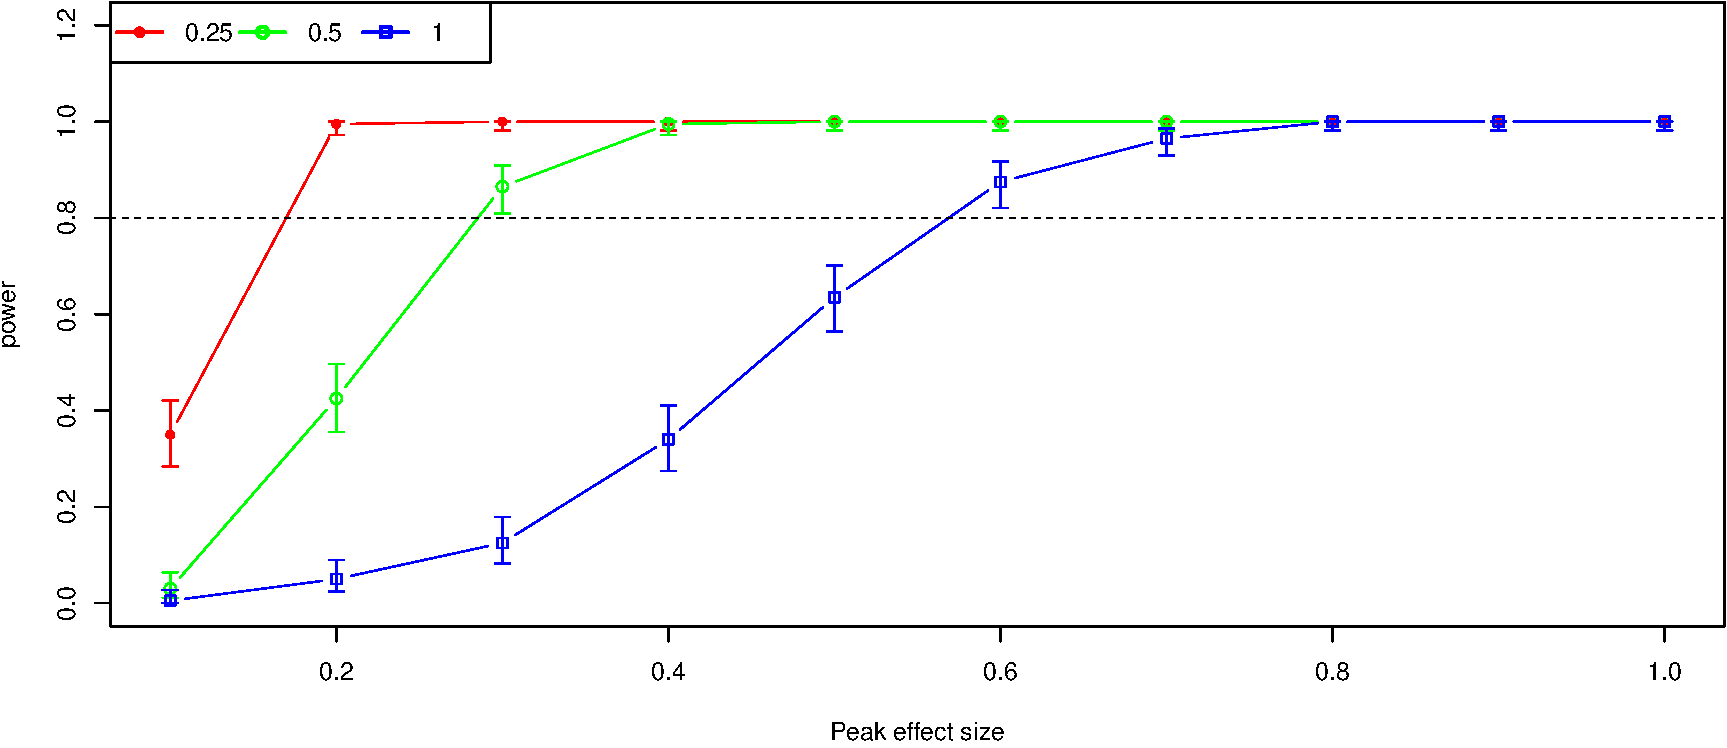
\includegraphics{power_calculations_files/figure-latex/esizes2-1.pdf}
\caption{Power as a function of peak effect size when fitting
polynomials to model time. Number of subjects is fixed at 120. The
different curves represent different within variance.}
\end{figure}

\section{Conclusions}\label{conclusions}

Except for the case with very low effect and high within variance, we
reach satisfactory power for the discussed sample sizes for the study
(at least 700 subjects).

For lower sample sizes (100-200) we still see a reasonable power for
high or medium effects as along as the within variance is not too high.


\end{document}
